\chapter{METODOLOGI PENELITIAN}
\section{Studi Literatur}
Studi literature dilakukan dengan mempelajari penelitian yang berkaitan dengan materi \emph{hand gesture recognition}, \emph{Retinex} dan \emph{Convolutional Neural Network} yang  diperoleh dari berbagai sumber seperti buku, artikel, jurnal dan sumber lain yang diperoleh dari internet.
\section{Alat dan Bahan}
\subsection{Alat}
Penelitian ini menggunakan beberapa peralatan yang digunakan untuk membantu kegiatandari mulai pengumpulan data hingga pengujian sistem, beberapa peralatan tersebut adalah sebagai berikut :
\begin{enumerate}
\item PC/Laptop dengan spesifikasi processor Intel (R) Core i5-8300H CPU @2,4 GHz, GPU NVIDIA 1050, RAM 8 GB, sistem operasi Linux 64 bit.
\item Webcam Logitech C270
\item Dimmer
\item Kain	
\item Lux Meter
\end{enumerate}
Laptop merupakan peralatan yang paling utama yang digunakan untuk melakukan proses pengolahan citra dengan webcam sebagai alat untuk menangkap citra. Lux meter digunakan untuk mengukur intensitas cahaya saat pengambilan data dan pengujian data dengan menurunkan intensitas cahaya yang diatur menggunakan dimmer. Penggunaan kain bersifat opsional untuk latar belakang yang bervariasi.
\subsection{Bahan}
Bahan yang digunakan untuk melakukan penelitian ini berupa dataset, diantaranya sebagai berikut:
\begin{enumerate}
	\item Dataset gestur tangan ASL 
	\item Dataset gambar tangan
\end{enumerate}
Dataset gestur tangan ASL merupakan dataset dari \emph{Massey University} yang digunakan untuk melatih model pengenalan gestur tangan, sementara dataset gambar tangan merupakan dataset untuk melakukan pelatihan deteksi tangan. Dataset gambar tangan diambil dari 3 subjek yang diambil gambar menggunakan webcam.
\section{Prosedur Kerja}
\subsection{Analisis dan Perancangan Sistem}
Alur penelitian yang akan dilakukan dalam penelitian ini memiliki beberapa tahapan diantaranya pengambilan dataset gestur, training data dan tahap paling akhir adalah pengujian. Alur kegiatan penelitian yang akan dilakukan secara garis besar ditunjukan pada Gambar 4.1.
% TODO: \usepackage{graphicx} required
\begin{figure}[H]
	\centering
	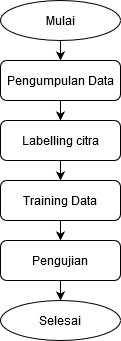
\includegraphics[width=0.2\linewidth]{Rencana}
	\caption{Alur Kegiatan Penelitian}
	\label{fig:screenshot006}
\end{figure}
Rancangan pengujian sistem ditunjukan pada Gambar 4.2 yang dimulai dengan \emph{input} dari webcam secara \emph{realtime}, sehingga setiap frame akan di proses pada tahap berikutnya.
Setiap frame dengan citra RGB akan dilewatkan pada algoritme \emph{Retinex} untuk dilakukan perbaikan kualitas citra dengan harapan meningkatkan kontras pada sebuah citra.
% TODO: \usepackage{graphicx} required
\begin{figure}[H]
	\centering
	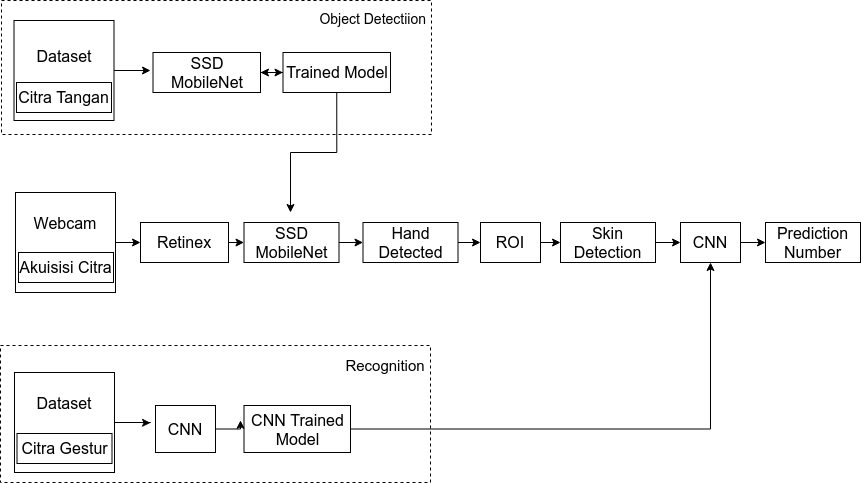
\includegraphics[width=1.1\linewidth]{rancanganedit}
	\caption{Rancangan Sistem}
	\label{fig:rancangan}
\end{figure}
\noindent Citra yang mengalami peningkatan kontras kemudian sistem akan melakukan deteksi tangan dengan \emph{SSD MobileNet} yang kemudian citra tangan tersebut akan diambil sebagai ROI. 
Citra hasil ROI akan dilakukan segmentasi menggunakan \emph{skin detection}. Hasil segmentasi akan diklasifikasikan dengan model CNN yang telah di training sebelumnya.
Keluaran dari sistem ini akan menampilkan klasifikasi angka yang terdeteksi.

Penelitian yang digambarkan pada rencana sistem memiliki 3 bagian penting diantaranya \emph{Retinex}, \emph{SSD MobileNet} dan \emph{Convolutional Neural Network}.
Peranan Retinex pada penelitian ini merupakan solusi untuk mengatasi permasalahan intensitas cahaya, sehingga pada dataset yang dilatih tidak perlu menggunakan variasi intensitas yang rendah. Penggunaan SSD dengan arsitektur \emph{MobileNet} bertujuan untuk mempercepat waktu komputasi supaya tidak terlalu berat dengan harapan lebih cepat. \emph{Convolutional Neural Network} sendiri digunakan untuk melakukan ekstraksi fitur dari sebuah citra. Ekstraksi fitur ini sangat sering digunakan dalam pemrosesan sebuah citra untuk memperoleh informasi. 
\subsection{Pra-proses}
Tahap pra-proses pada penelitian ini terdapat pada proses \emph{enhancement} yang dilakukan oleh \emph{Retinex}. Citra dengan intensitas cahaya rendah akan dilakukan proses perbaikan dahulu sebelum dilakukan proses deteksi maupun pengenalan. \emph{Input} citra untuk proses \emph{Retinex} menggunakan 3 kanal(R,G,B).

Proses pertama yang dilakukan adalah membuat filter \emph{gaussian} menggunakan Persamaan 3.14 dengan permisalan $\sigma$ = 10.

\noindent
$\left[
\begin{matrix}
	\frac{1}{2\pi(10)^2}\times \exp^{-\frac{(-1)^2+1^2}{2(10)^2}} & \frac{1}{2\pi(10)^2}\times \exp^{-\frac{0^2+1^2}{2(10)^2}} &\frac{1}{2\pi(10)^2}\times \exp^{-\frac{1^2+1^2}{2(10)^2}} \\
	\frac{1}{2\pi(10)^2}\times \exp^{-\frac{(-1)^2+0^2}{2(10)^2}} & \frac{1}{2\pi(10)^2}\times \exp^{-\frac{0^2+0^2}{2(10)^2}} &\frac{1}{2\pi(10)^2}\times \exp^{-\frac{1^2+0^2}{2(10)^2}} \\
	\frac{1}{2\pi(10)^2}\times \exp^{-\frac{(-1)^2+(-1)^2}{2(10)^2}} & \frac{1}{2\pi(10)^2}\times \exp^{-\frac{0^2+(-1)^2}{2(10)^2}} &\frac{1}{2\pi(10)^2}\times \exp^{-\frac{1^2+(-1)^2}{2(10)^2}} 	
\end{matrix}
\right]$

\noindent Filter \emph{gaussian} yang dihasilkan menggunakan $\sigma$=10 adalah sebagai berikut.

\noindent
$\left[
\begin{matrix}
	0,001575 & 0,001583 & 0,001575
	 \\
	0,001583 & 0,001591 & 0,001583
	\\
	0,001575 & 0,001583 & 0,001575
\end{matrix}
\right]$

\noindent Berdasarkan Persamaan 3.15, integral dari filter \emph{gaussian} harus sama dengan 1. Integral dari filter tersebut dapat dicari dengan menjumlahkan semua elemen. Pada kasus ini nilai integral atau jumlahan dari elemen adalah 0.0142288. Apabila hasil dari integral tersebut tidak sama dengan 1 maka akan dikalikan menggunakan formula berikut.\\
$
new\_a_{(x,y)}=a_{(x,y)}\times\frac{1}{total}
$\\
$
new\_a_{(-1,1)}=0,001575\times\frac{1}{0,142288}=0,110740\\
new\_a_{(-1,0)}=0,001583\times\frac{1}{0,142288}=0,111295
$

\noindent Perhitungan nilai filter \emph{gaussian} dilakukan untuk setiap distribusi kernel sehingga membentuk filter dengan nilai baru. Nilai filter yang baru menghasilkan hasil integral sama dengan 1.\\

\noindent
$\left[
\begin{matrix}
0,110740&0,111295&0,110740\\
0,111295&0,111853&0,111295\\
0,110740&0,111295&0,110740
\end{matrix}
\right]$

\noindent Filter \emph{gaussian} ini akan dikonvolusikan dengan input citra, contoh citra yang akan dikonvolusikan sebagai berikut.

\noindent
$I_{(x,y)}=\left[
\begin{matrix}
0&0&0&0&0&0\\
0&120&	125&	124&	126&0\\
0&126&	135&	146&	189&0\\
0&170&	187&	200&	210&0\\
0&189&	188&	197&	221&0\\
0&0&0&0&0&0
\end{matrix}
\right]$*
$F_{(x,y)}=\left[
\begin{matrix}
0,110740 &0,111295&0,110740\\
0,111295&0,111853&0,111295\\
0,110740&0,111295&0,110740\\
\end{matrix}
\right]$

\noindent Perhitungan konvolusi untuk mendapatkan dimensi yang sama dengan citra \emph{input} digunakan \emph{zero padding}. Hasil konvolusi di ilustrasikan pada perhitungan berikut.

\noindent $O_{(1,1)}=$(0*0,110740)+(0*0.111295)+(0*0,110740)+(0*0,111295)+(120*0,111853)\\
+(125*0,111295)+(0*0,110740)+(126*0,111295)+(135*0,110740)=56,307698

\noindent$O_{(2,1)}=$(0*0,110740)+(0*0,111295)+(0*0,110740)+(120*0,111295)+(125*0,111853)\\
+(124*0,111295)+(126*0,110740)+(135*0,111295)+(146*0,110740)=86,284315

\noindent Konvolusi dilakukan dengan pergeseran 1 piksel sehingga menghasilkan citra dengan dimensi yang sama. Hasil konvolusi($O_{(x,y)}$) merupakan nilai dari Persamaan 3.13 yang mendapatan nilai sebagai berikut.

\noindent
$O_{(x,y)}=\left[
\begin{matrix}
56,307698&	86,284315&	93,934305&	65,097310\\
95,945406&	148,09183&	160,21034&	110,66494\\
110,65489&	170,91206&	185,90262&	129,36380\\
81,692776&	125,77508&	133,77841&	92,165220
\end{matrix}
\right]$\\
$\log O_{(x,y)}=\left[
\begin{matrix}
1,750568&	1,935932&	1,972825&	1,813563\\
1,982024&	2,170531&	2,204691&	2,044011\\
2,043971&	2,232773&	2,269286&	2,111813\\
1,912183&	2,099594&	2,126386&	1,964568

\end{matrix}
\right]$

\noindent Nilai akhir dari \emph{Single Scale Retinex} adalah pengurangan antara hasil logaritmik citra asli dengan logaritmik citra hasil konvolusi dimana dituliskan dalam Persamaan 3.17. Berikut adalah hasil \emph{Single Scale Retinex}($\sigma$=10).

\noindent
$R_{(SSR(\sigma=10))=}\left[
\begin{matrix}
0,328612&	0,160977&	0,120596&	0,286806\\
0,118345&	-0,040198&	-0,04033&	0,232450\\
0,186477&	0,039068&	0,031743&	0,210405\\
0,364278&	0,174563&	0,168079&	0,379824
\end{matrix}
\right]$

\noindent Perhitungan \emph{Multiscale Retinex} jumlahan dari setiap \emph{Single Scale Retinex}. \emph{Single Scale Retinex} dengan $\sigma$=65 dan $\sigma$=180 didapatkan nilai sebagai berikut.

\noindent
$R_{(SSR(\sigma=65))=}\left[
\begin{matrix}
0,329257&	0,161283&	0,120802&	0,287442\\
0,118596&	-0,040252&	-0,040368&	0,232871\\
0,186859&	0,039126&	0,031776&	0,210871\\
0,364991&	0,174929&	0,168434&	0,380586
\end{matrix}
\right]$

\noindent
$R_{(SSR(\sigma=180))=}\left[
\begin{matrix}
0,329271&	0,161289&	0,120806&	0,287455\\
0,118601&	-0,040253&	-0,040369&	0,232879\\
0,186867&	0,0391275&	0,0317764&	0,210880\\
0,365006&	0,1749365&	0,1684419&	0,380602
\end{matrix}
\right]$

\noindent \emph{Multiscale Retinex} memiliki bobot pada setiap skala, dimana jika bobot dijumlahkan = 1. Bobot tersebut dikalikan dengan citra untuk masing masing skala, sehingga mendapatkan nilai berikut dengan masing masing bobot$\omega_n=0.3, 0.3, 0.4$.

\noindent
$R_{(SSR(\sigma=10))*0,3}\left[
\begin{matrix}
0,098583&	0,048293&	0,036178&	0,086041\\
0,035503&	-0,012059&	-0,012101&	0,069735\\
0,055943&	0,011720&	0,009523&	0,063121\\
0,109283&	0,052368&	0,050423&	0,113947
\end{matrix}
\right]$

\noindent
$R_{(SSR(\sigma=65))*0,3}\left[
\begin{matrix}
0,098777&	0,048385&	0.036240&	0.086232\\
0,035578&	-0,012075&	-0.012110&	0.069861\\
0,056057&	0,011737&	0.009532&	0.063261\\
0,109497&	0,052478&	0.050530&	0.114175
\end{matrix}
\right]$

\noindent
$R_{(SSR(\sigma=180))*0,4}\left[
\begin{matrix}
0,131708&	0,064515&	0,048322&	0,114982\\
0,047440&	-0,016101&	-0,016147&	0,093151\\
0,074746&	0,015651&	0,012710&	0,084352\\
0,146002&	0,069974&	0,067376&	0,152240
\end{matrix}
\right]$

\noindent Setiap nilai \emph{Single Scale Retinex} dijumlahkan seperti pada Persamaan 3.18, kemudian hasil dari penjumlahan akan dilakukan normalisasi dengan hasil akhir yang dibulatkan.

\noindent
$R_{(MSR)}=\left[
\begin{matrix}
0,329069&	0,161194&	0,120742&	0,287256\\
0,118523&	-0,040236&	-0,040360&	0,232748\\
0,186748&	0,039109&	0,031766&	0,210735\\
0,364783&	0,174822&	0,168331&	0,380363
\end{matrix}
\right]$

\noindent Normalisasi = $\frac{(ABS(Nilai_{(x,y)})-Nilai\_min)}{(Nilai\_max-Nilai\_min)}$$\times$255

\noindent
$R_{(MSR)}=\left[
\begin{matrix}
224&	122&	98&		198\\
96&		0&		1&		165\\
138&	48&		44&		152\\
246&	130&	126&	255

\end{matrix}
\right]$\\
Gambar 4.3 menunjukan ilustrasi peningkatan kualitas citra dengan intensitas cahaya rendah dikenai algoritme \emph{retinex} sehingga menghassilkan citra dengan pengingkatan kontras.
% TODO: \usepackage{graphicx} required
\begin{figure}[H]
	\centering
	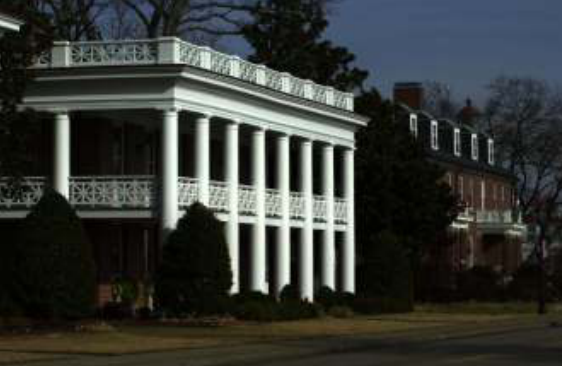
\includegraphics[width=0.4\linewidth]{ret1}
	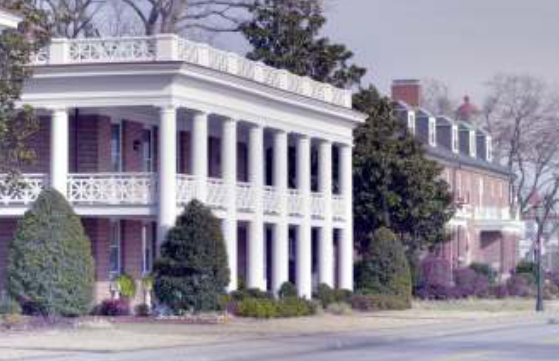
\includegraphics[width=0.4\linewidth]{ret2}\\
	a \ \ \ \ \ \ \ \ \ \ \ \ \ \ \ \ \ \ \ \  \ \ \ \ \ \ \ \ \ \ \ \ \ \ \ \ \ \ \ \ \ \ \ \ \ \ \ \ \ \ \ \ b
	\caption{Ilustrasi Perbaikan Kontras Menggunakan Retinex (a) Citra Asli; (b) Citra Hasil Perbaikan(Petro et al., 2014)}
	\label{fig:ret1}
	\label{fig:ret2}
\end{figure}


\subsection{Pengumpulan Data}
Data pelatihan dibagi menjadi dua, yaitu dataset citra gestur tangan yang mengacu pada ASL dan dataset citra tangan biasa untuk \emph{object detection}.
Kedua dataset ini merupakan dua hal yang berbeda tujuan. 
Dataset ASL digunakan untuk model pengenalan gestur ASL dan dataset citra tangan digunakan untuk model deteksi tangan.

Dataset gestur tangan ASL menggunakan dataset public dari \emph{Massey University}. Dataset tersebut berisi 2425 citra yang dibagai dalam 36 kelas, yaitu 26 untuk huruf A-Z dan 10 kelas untuk angka 0-9. Pengambilan dataset dilakukan oleh 5 individu dengan variasi cahaya yang berbeda(Barczak et al., 2011).
Acuan dalam penelitian ini menggunakan dataset angka 0 sampai 9, dengan citra yang sudah di segmentasi.
Dataset ini akan dilatih dalam CNN untuk pengenalan gestur tangan.
Pengambilan dataset \emph{Massey University} dilakukan menggunakan \emph{green screen} sehingga mudah untuk disegmentasi, setup pengambilan dataset dilakukan dengan skema seperti Gambar 4.4 (Barczak et al., 2011).

Pengambilan dataset berikutnya berbeda dengan dataset ASL, dataset berikutnya diambil menggunakan webcam untuk keperluan deteksi tangan, citra diambil dari 10 orang dengan random pose. Dataset ini digunakan untuk pelatihan pada \emph{object detection}. 
Pengambilan dataset dilakukan masing masing 100 capture untuk setiap orang, sehingga pada dataset ini diperoleh 1000 citra. 

Proses pengumpulan dataset tidak menghiraukan nilai intensitas cahaya karena permasalahan pencahayaan sudah diatasi pada algoritme \emph{Retinex}, namun akan tetap diukur kondisi intensitas pada lingkungan tersebut menggunakan lux meter. Penggunaan dataset ASL dari \emph{Massey University} tidak memiliki keterangan nilai intesitas cahaya, namun berdasarkan citra tersebut cenderung memiliki nilai intensitas yang tinggi, dimana dapat dilihat pada isi dataset. Tujuan dari dataset yang dilatih hanya untuk membuat model klasifikasi dan deteksi tanpa memperhitungkan intensitas cahaya rendah.
% TODO: \usepackage{graphicx} required
\begin{figure}[H]
	\centering
	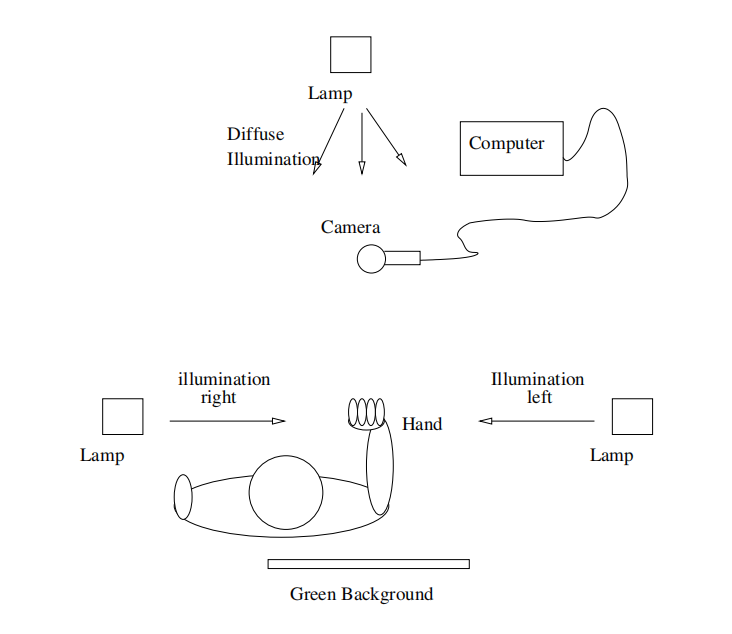
\includegraphics[width=0.8\linewidth]{setup}
	\caption{Skema Pengambilan Dataset (Barczak et al., 2011)}
	\label{fig:setup}
\end{figure}
\section{Proses Pelatihan}
Proses pelatihan dalam penelitian ini dibagi menjadi dua bagian, yaitu pelatihan object detection dan pelatihan gestur recognition.
\subsection{Pelatihan Gesture Recognition}
Dataset pada pelatihan \emph{gesture recognition} menggunakan dataset dari \emph{Massey Univertisy} yang di labeli sesuai acuan ASL dari angka 0 hingga 9. Jumlah dataset adalah 700 citra kemudian dibagi yang akan dibagi dalam \emph{train} dan \emph{test} menggunakan \emph{k-fold cross validation} dengan k = 5.
Proses pelatihan untuk pengenalan gestur tangan menggunakan teknik \emph{transfer learning} yang memiliki kelebihan pada waktu pelatihan dan penggunaan dataset yang cenderung sedikit. \emph{Pre-trained} model yang digunakan adalah \emph{MobileNetV2}. \emph{Pre-trained} model memiliki pengetahuan dari dataset yang telah dilatih sebelumnya, pada \emph{MobileNetV2} telah dilatih menggunakan dataset dari \emph{ImageNet}, kemudian pengetahuan tersebut akan di pindahkan ke model baru dan dilatih sesuai dataset baru, sehingga memiliki keluaran dalam bentuk klasifikasi atau tugas sesuai yang diinginkan.

Masukan citra memiliki dimensi 224x224 piksel yang terdiri 3 channel RGB, sehingga node \emph{input} berjumlah 50176 dengan range 0-255 untuk setiap piksel. Arsitektur jaringan pada pelatihan ini dilakukan dengan mengganti bagian blok klasifikasi dari \emph{MobileNetV2} menjadi klasifikasi dataset ASL. 
Arsitektur transfer learning dapat dilihat pada Gambar 4.5.
% TODO: \usepackage{graphicx} required
\begin{figure}[H]
	\centering
	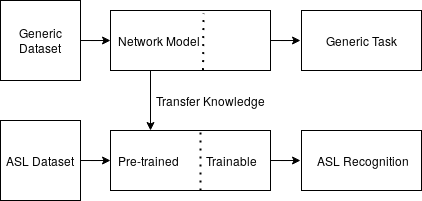
\includegraphics[width=0.8\linewidth]{transfer}
	\caption{Transfer Learning Pelatihan Gestur}
	\label{fig:asritrkturku}
\end{figure}

\subsection{Pelatihan Object Detection}
Proses pelatihan pada \emph{object detection} menggunakan \emph{pre-trained model SSD MobilenetV2 COCO} yang sudah di latih sebelumnya dengan dataset COCO.
Dataset yang baru akan dilatih menggunakan \emph{pre-trained} model, sehingga dengan pengetahuan yang sudah ada dilatih agar menghasilkan model baru sesuai dengan \emph{output} yang diinginkan. 
Dataset yang akan dilatih sejumlah 1000 citra yang telah dilabeli secara manual dengan pembagian 80\% \emph{training} dan 20\% \emph{testing}.
Arsitektur yang digunakan dalam pelatihan \emph{object detection} dapat dilihat pada Gambar 4.6.
\begin{figure}[H]
	\centering
	\includegraphics[width=0.7\linewidth]{"v2"}
	\caption{Arsitektur Mobilenet V2 (Sandler et al., 2018)}
	\label{fig:v2}
\end{figure}
%----------------------------------PENGUJIAN-------------------------------------
\section{Pengujian dan Evaluasi}
Pengujian dan evaluasi adalah tahap untuk mengukur performa dari sebuah sistem. Pengujian ini akan dibagi menjadi 6 tahap, yaitu evaluasi deteksi tangan, evaluasi pengenalan gestur, pengujian deteksi tangan menggunakan \emph{Retinex}, pengujian pengenalan gestur tangan menggunakan \emph{Retinex}, pengujian SNR dan pengujian keseluruhan sistem. 
Setiap pengujian yang menggunakan Retinex dilakukan hal yang sama, yaitu dengan menurunkan intensitas cahaya.
%------------------------------------PENGUJIAN DETEKSI------------------------
\subsection{Evaluasi Deteksi Tangan}
Evaluasi model deteksi tangan dilakukan setelah \emph{training} menggunakan metrik \emph{mean average precicion} (mAP). \emph{Mean average precicion} merupakan metrik yang populer untuk mengevaluasi model dari detektor. \emph{Mean average precicion} merupakan rata rata dari \emph{Average Precicion} (AP) pada setiap nilai IoU. Sesuai dengan acuan COCO dataset untuk mengevaluasi model pada \emph{object detection} dengan menghitung mAP dari IoU=0,5 hingga 0,95 dengan pertambahan 0,05.
\subsection{Evaluasi Pengenalan Gestur Tangan}
Evaluasi model CNN untuk pengenalan gestur tangan didapatkan saat \emph{training} dan \emph{testing} menggunakan \emph{k-fold cross validation} dengan k = 5, dimana dilakukan validasi sebanyak 5 kali dengan skenario pengujian yang berbeda pada proses \emph{training} dan \emph{testing}.
\emph{Training accuracy} dan \emph{testing accuracy} didapatkan pada setiap \emph{fold}. Model dengan akurasi terdinggi akan digunakan sebagai model untuk pengenalan gestur tangan.
\subsection{Pengujian SNR}
SNR\emph{(Signal to Noise Ratio)} adalah ukuran untuk mengukur kualitas citra terhadap citra yang dilakukan perbaikan. Citra hasil perbaikan dibandingkan dengan citra asli untuk mendapatkan nilai SNR nya. Nilai SNR yang tinggi mengindikasikan kualitas citra yang semakin baik karena rasio sinyal terhadap metode juga tinggi, sebaliknya nilai SNR yang rendah berarti kualitas citra yang di hasilkan semakin buruk atau semakin kecil dalam peningkatan kualitas citra. Pengujian SNR ini dilakukan untuk menentukan nilai dari parameter \emph{retinex} yang akan dipakai pada sistem.
\subsection{Pengujian Deteksi Tangan Menggunakan Retinex}
Tujuan pengujian deteksi tangan dilakukan untuk menguji sistem dalam melakukan deteksi tangan terkait dengan penurunan intensitas cahaya. Ilustrasi pengujian deteksi tangan digambarkan pada Gambar 4.7. Pengujian dilakukan dengan kondisi cahaya awal sesuai yang terjadi pada ruangan. Pada kondisi awal tersebut akan dilakukan deteksi tangan, setiap hasil dari deteksi tersebut berupa \emph{true positive} atau \emph{false positive}. Hasil deteksi akan dicatat dalam bentuk tabel seperti pada Tabel 4.1.
% TODO: \usepackage{graphicx} required
\begin{figure}[H]
	\centering
	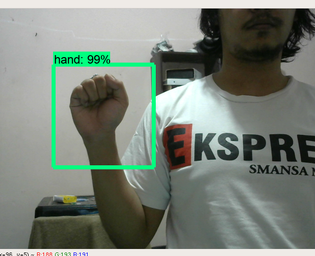
\includegraphics[width=0.72\linewidth]{deteksihand}
	\caption{Ilustrasi Pengujian Deteksi Tangan}
	\label{fig:deteksihand}
\end{figure}
% TODO: \usepackage{graphicx} required
\begin{figure}[H]
	\centering
	\includegraphics[width=0.4\linewidth]{"skema pengujian deteksi tangan"}
	\caption{Skema Kegiatan Pengujian Deteksi Tangan}
	\label{fig:skema-objek-deteksi}
\end{figure}
Pada pengujian ini alur kegiatan yang dilakukan saat pengujian deteksi tangan dapat dilihat pada Gambar 4.8. Pengujian deteksi tangan dilakukan secara manual oleh 3 subjek yang berbeda, setiap subjek akan dicatat apakah sistem mampu mendeteksi tangan atau tidak pada intensitas cahaya pada saat itu selama 10 kali, kemudian dilakukan penurunan intensitas sebesar 50\% untuk kondisi selanjutnya dan dilakukan hal yang sama. Penurunan ini dilakukan hingga nilai lux yang terukur bernilai kurang dari atau sama dengan 50lux. Evaluasi pengujian dilakukan dengan \emph{confussion matrix} menggunakan data yang dicatat pada Tabel 4.1, sehingga dapat diperoleh nilai akurasi untuk setiap kondisi lux dari hasil pengujian.
\begin{table}[H]
	\caption{Pengujian Deteksi Tangan}
	\vspace{0cm}
	\centering
	\begin{tabular}{|c|c|c|c|c|c|c|c|c|c|c|c|c|c|c|c|c|c|c|c|c|c|c|c|c|c|c|c|c|c|c|}
		\hline
		Nilai Lux(X) & \multicolumn{10}{|c|}{Hasil Deteksi Subjek\_1} & \multicolumn{10}{|c|}{Hasil Deteksi Subjek\_2}& \multicolumn{10}{|c|}{Hasil Deteksi Subjek\_3}\\
		\hline X & & & &&&&&&&&&&&&&&&&&&&&&&&&&&&\\
		\hline X=X*50\% & & & &&&&&&&&&&&&&&&&&&&&&&&&&&&\\
		\hline X=X*50\% & & & & && &&&&&&&&&&&&&&&&&&&&&&&&\\
		\hline X=X*50\% & & & &&&&&&& &&&&&&&&&&&&&&&&&&&&\\
		\hline $\dots$ & & & & & &&&&&&&&&&&&&&&&&&&&&&&&&\\
		\hline X=X $\le$ 50Lux & & & &&&&&&& &&&&&&&&&&&&&&&&&&&&\\
		\hline
	\end{tabular}
\end{table}
%------------------------------PENGUJIAN GESTUR------------------------------------
\subsection{Pengujian Pengenalan Gestur Tangan Menggunakan Retinex}
Pengujian tahap kedua yaitu pengenalan gestur tangan dengan \emph{retinex}. Tujuan dari pengujian ini untuk mengukur performa sistem dalam melakukan pengenalan gestur tangan dengan acuan ASL sesuai dengan dataset yang telah dilatih. Skema kegiatan pengujian pengenalan gestur tangan dapat dilihat pada Gambar 4.9.
Pengujian dilakukan dengan kondisi cahaya awal sesuai yang terjadi pada ruangan. Pada kondisi awal tersebut akan dilakukan pengenalan gestur tangan, setiap hasil dari pengenalan tersebut berupa \emph{true positive} atau \emph{false positive}. Nilai \emph{true positive} terjadi apabila \emph{input} gestur tangan dari webcam sesuai dengan klasifikasi gestur tangan ASL yang sebenarnya. Nilai \emph{false positive} terjadi apabila \emph{input} gestur tangan tidak sesuai dengan klasifikasi gestur ASL yang sebenarnya. Hasil pengenalan akan dicatat dalam bentuk tabel seperti pada Tabel 4.1.
% TODO: \usepackage{graphicx} required
\begin{figure}[H]
	\centering
	\includegraphics[width=0.4\linewidth]{"skema pengujian pengenalan tangan"}
	\caption{Skema Kegiatan Pengujian Pengenalan Gestur Tangan}
	\label{fig:screenshot-from-2020-03-04-22-24-45}
\end{figure}

% TODO: \usepackage{graphicx} required
\begin{figure}[H]
	\centering
	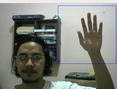
\includegraphics[width=0.5\linewidth]{recoghand}
	\caption{Ilustrasi Pengujian Pengenalan Gestur Tangan}
	\label{fig:recoghand}
\end{figure}
Ilustrasi pengujian ini digambarkan pada Gambar 4.10. Pengujian pengenalan gestur tangan dilakukan secara manual dan terpisah dari deteksi tangan, tahap ini memiliki perlakuan sama dengan tahap sebelumnya, yaitu menggunakan 3 subjek yang berbeda, kemudian dilakukan pengenalan gestur tangan sebanyak 10 kali untuk setiap klasifikasi. Total citra yang didapat dalam satu kondisi lux oleh satu subjek adalah 100 citra.
Tahap berikutnya dilakukan penurunan intensitas cahaya, dengan mengatur cahaya lampu di ruangan uji sebesar 50\% lux menggunakan dimmer. Pengujian dilakukan hingga batas lux kurang dari atau sama dengan 50 lux. Evaluasi yang dilakukan dengan \emph{confussion matrix} menggunakan data yang diperoleh pada Tabel 4.2. Hasil evaluasi pengujian akan diperoleh nilai akurasi untuk setiap kondisi lux. 
\begin{table}[H]
	\caption{Pengujian Pengenalan Gestur Tangan}
	\vspace{0cm}
	\centering
\begin{tabular}{|c|}
	\hline
	\multicolumn{1}{|c|}{Nilai Lux(X)}\\

	\begin{tabular}{|c|c|c|c|c|c|c|c|c|c|c|c|c|c|c|c|c|c|c|c|c|c|c|c|c|c|c|c|c|c|c|c|c|}
		\hline
		Klasifikasi & \multicolumn{10}{|c|}{Pengenalan Subjek\_1}& \multicolumn{10}{|c|}{Pengenalan Subjek\_2}& \multicolumn{10}{|c|}{Pengenalan Subjek\_3}\\
		\hline Angka 0 & & & &&&&&&&&&&&&&&&&&&&&&&&&&&&\\
		\hline Angka 1 & & & &&&&&&&&&&&&&&&&&&&&&&&&&&&\\
		\hline Angka 2 & & & & && &&&&&&&&&&&&&&&&&&&&&&&&\\
		
		\hline ... & & & &&&&&&&&&&&&&&&&&&&&&&&&&&& \\
		\hline Angka 9 & & & &&&&&&&&&&&&&&&&&&&&&&&&&&& \\
		\hline
	\end{tabular}
\end{tabular}
%%======================================================
\begin{tabular}{|c|}
	\multicolumn{1}{|c|}{Nilai Lux(...)}\\	
	\begin{tabular}{|c|c|c|c|c|c|c|c|c|c|c|c|c|c|c|c|c|c|c|c|c|c|c|c|c|c|c|c|c|c|c|c|c|}
		\hline
		Klasifikasi & \multicolumn{10}{|c|}{Pengenalan Subjek\_1}& \multicolumn{10}{|c|}{Pengenalan Subjek\_2}& \multicolumn{10}{|c|}{Pengenalan Subjek\_3}\\
		\hline Angka 0 & & & &&&&&&&&&&&&&&&&&&&&&&&&&&&\\
		\hline Angka 1 & & & &&&&&&&&&&&&&&&&&&&&&&&&&&&\\	
		\hline Angka 2 & & & &&&&&&&&&&&&&&&&&&&&&&&&&&&\\	
		\hline ... & & & &&&&&&&&&&&&&&&&&&&&&&&&&&& \\
		\hline Angka 9 & & & &&&&&&&&&&&&&&&&&&&&&&&&&&& \\
		\hline
	\end{tabular}	
\end{tabular}
%%======================================================
\begin{tabular}{|c|}

	\multicolumn{1}{|c|}{Nilai Lux(X$\le$50)}\\
	\begin{tabular}{|c|c|c|c|c|c|c|c|c|c|c|c|c|c|c|c|c|c|c|c|c|c|c|c|c|c|c|c|c|c|c|c|c|}
		\hline
		Klasifikasi & \multicolumn{10}{|c|}{Pengenalan Subjek\_1}& \multicolumn{10}{|c|}{Pengenalan Subjek\_2}& \multicolumn{10}{|c|}{Pengenalan Subjek\_3}\\
		\hline Angka 0 & & & &&&&&&&&&&&&&&&&&&&&&&&&&&&\\
		\hline Angka 1 & & & &&&&&&&&&&&&&&&&&&&&&&&&&&&\\	
		\hline Angka 2 & & & &&&&&&&&&&&&&&&&&&&&&&&&&&&\\
		\hline ... & & & &&&&&&&&&&&&&&&&&&&&&&&&&&& \\
		\hline Angka 9 & & & &&&&&&&&&&&&&&&&&&&&&&&&&&& \\
		\hline
	\end{tabular}
\end{tabular}
\end{table}
\subsection{Pengujian Sistem Keseluruhan}
Pengujian tahap terakhir adalah pengujian keseluruhan sistem yang dilakukan secara manual, dengan menggabungkan \emph{retinex}, deteksi tangan dan pengenalan gestur tangan dalam satu program utuh. Pengenalan akan terjadi apabila sebuah tangan dideteksi terlebih dahulu, jika tidak terdeteksi maka tidak akan dilakukan pengenalan. Nilai yang didapatkan dari hasil pengujian ini berupa \emph{true positive} dan \emph{false positive}. \emph{True positive} didapatkan ketika sebuah \emph{input} citra gestur dari webcam menghasilkan klasifikasi ASL yang sama dengan gestur ASL yang sebenarnya. Nilai \emph{false positive} terjadi apabila \emph{input} citra gestur dari webcam menghasilkan klasifikasi yang tidak sesuai dengan gestur ASL yang sebenarnya.

Penurunan intensitas dilakukan sama seperti pengujian sebelumnya. Tabel pengujian yang digunakan mengacu pada Tabel 4.2. Evaluasi dari akurasi sistem keseluruhan dapat diperoleh menggunakan \emph{confusion matrix} pada data yang dicatat pada tabel. Nilai akurasi dihitung untuk setiap kondisi lux yang tercatat pada tabel pengujian.